\section{Une propriété géométique de l'intégrale}

\begin{exercice}
    Soit $f$ de classe $\mathscr{C}^1$ sur $[a, b]$ telle que $f'$ soit strictement positive sur $[a, b]$. Calculer:
    $$\int_{a}^{b} f(t) \d t + \int_{f(a)}^{f(b)} f^{-1}(t) \d t.$$
\end{exercice}

\begin{elem_sol}
    \begin{enumerate}
    \item Comme $f' > 0$, alors $f$ est strictement croissante. Comme $f$ est continue, d'après le théorème de la bijection monotone, $f$ réalise une bijection de $[a, b]$ sur $[f(a), f(b)]$.
    
    \item On utilise le changement de variable $\phi : [a, b] \to [f(a), f(b)],\, u \mapsto f(u)$. Alors, $\phi$ est de classe $\mathscr{C}^1$ et
    \begin{align*}
    \int_{f(a)}^{f(b)} f^{-1}(t) \d t
    &= \int_a^b f^{-1}(f(u)) f'(u) \d u\\
    &= \int_a^b u f'(u) \d u\\
    &= \left[u f(u)\right]_a^b - \int_a^b f(u) \d u,
    \end{align*}
    où on a réalisé une intégration par parties.
    \end{enumerate}

    Finalement,
    \[
    \int_a^b f(t) \d t + \int_{f(a)}^{f(b)} f^{-1}(t) \d t = b f(b) - a f(a).
    \]
\end{elem_sol}



% \todoinline{Une version plus claire de mon dessin ?}

% 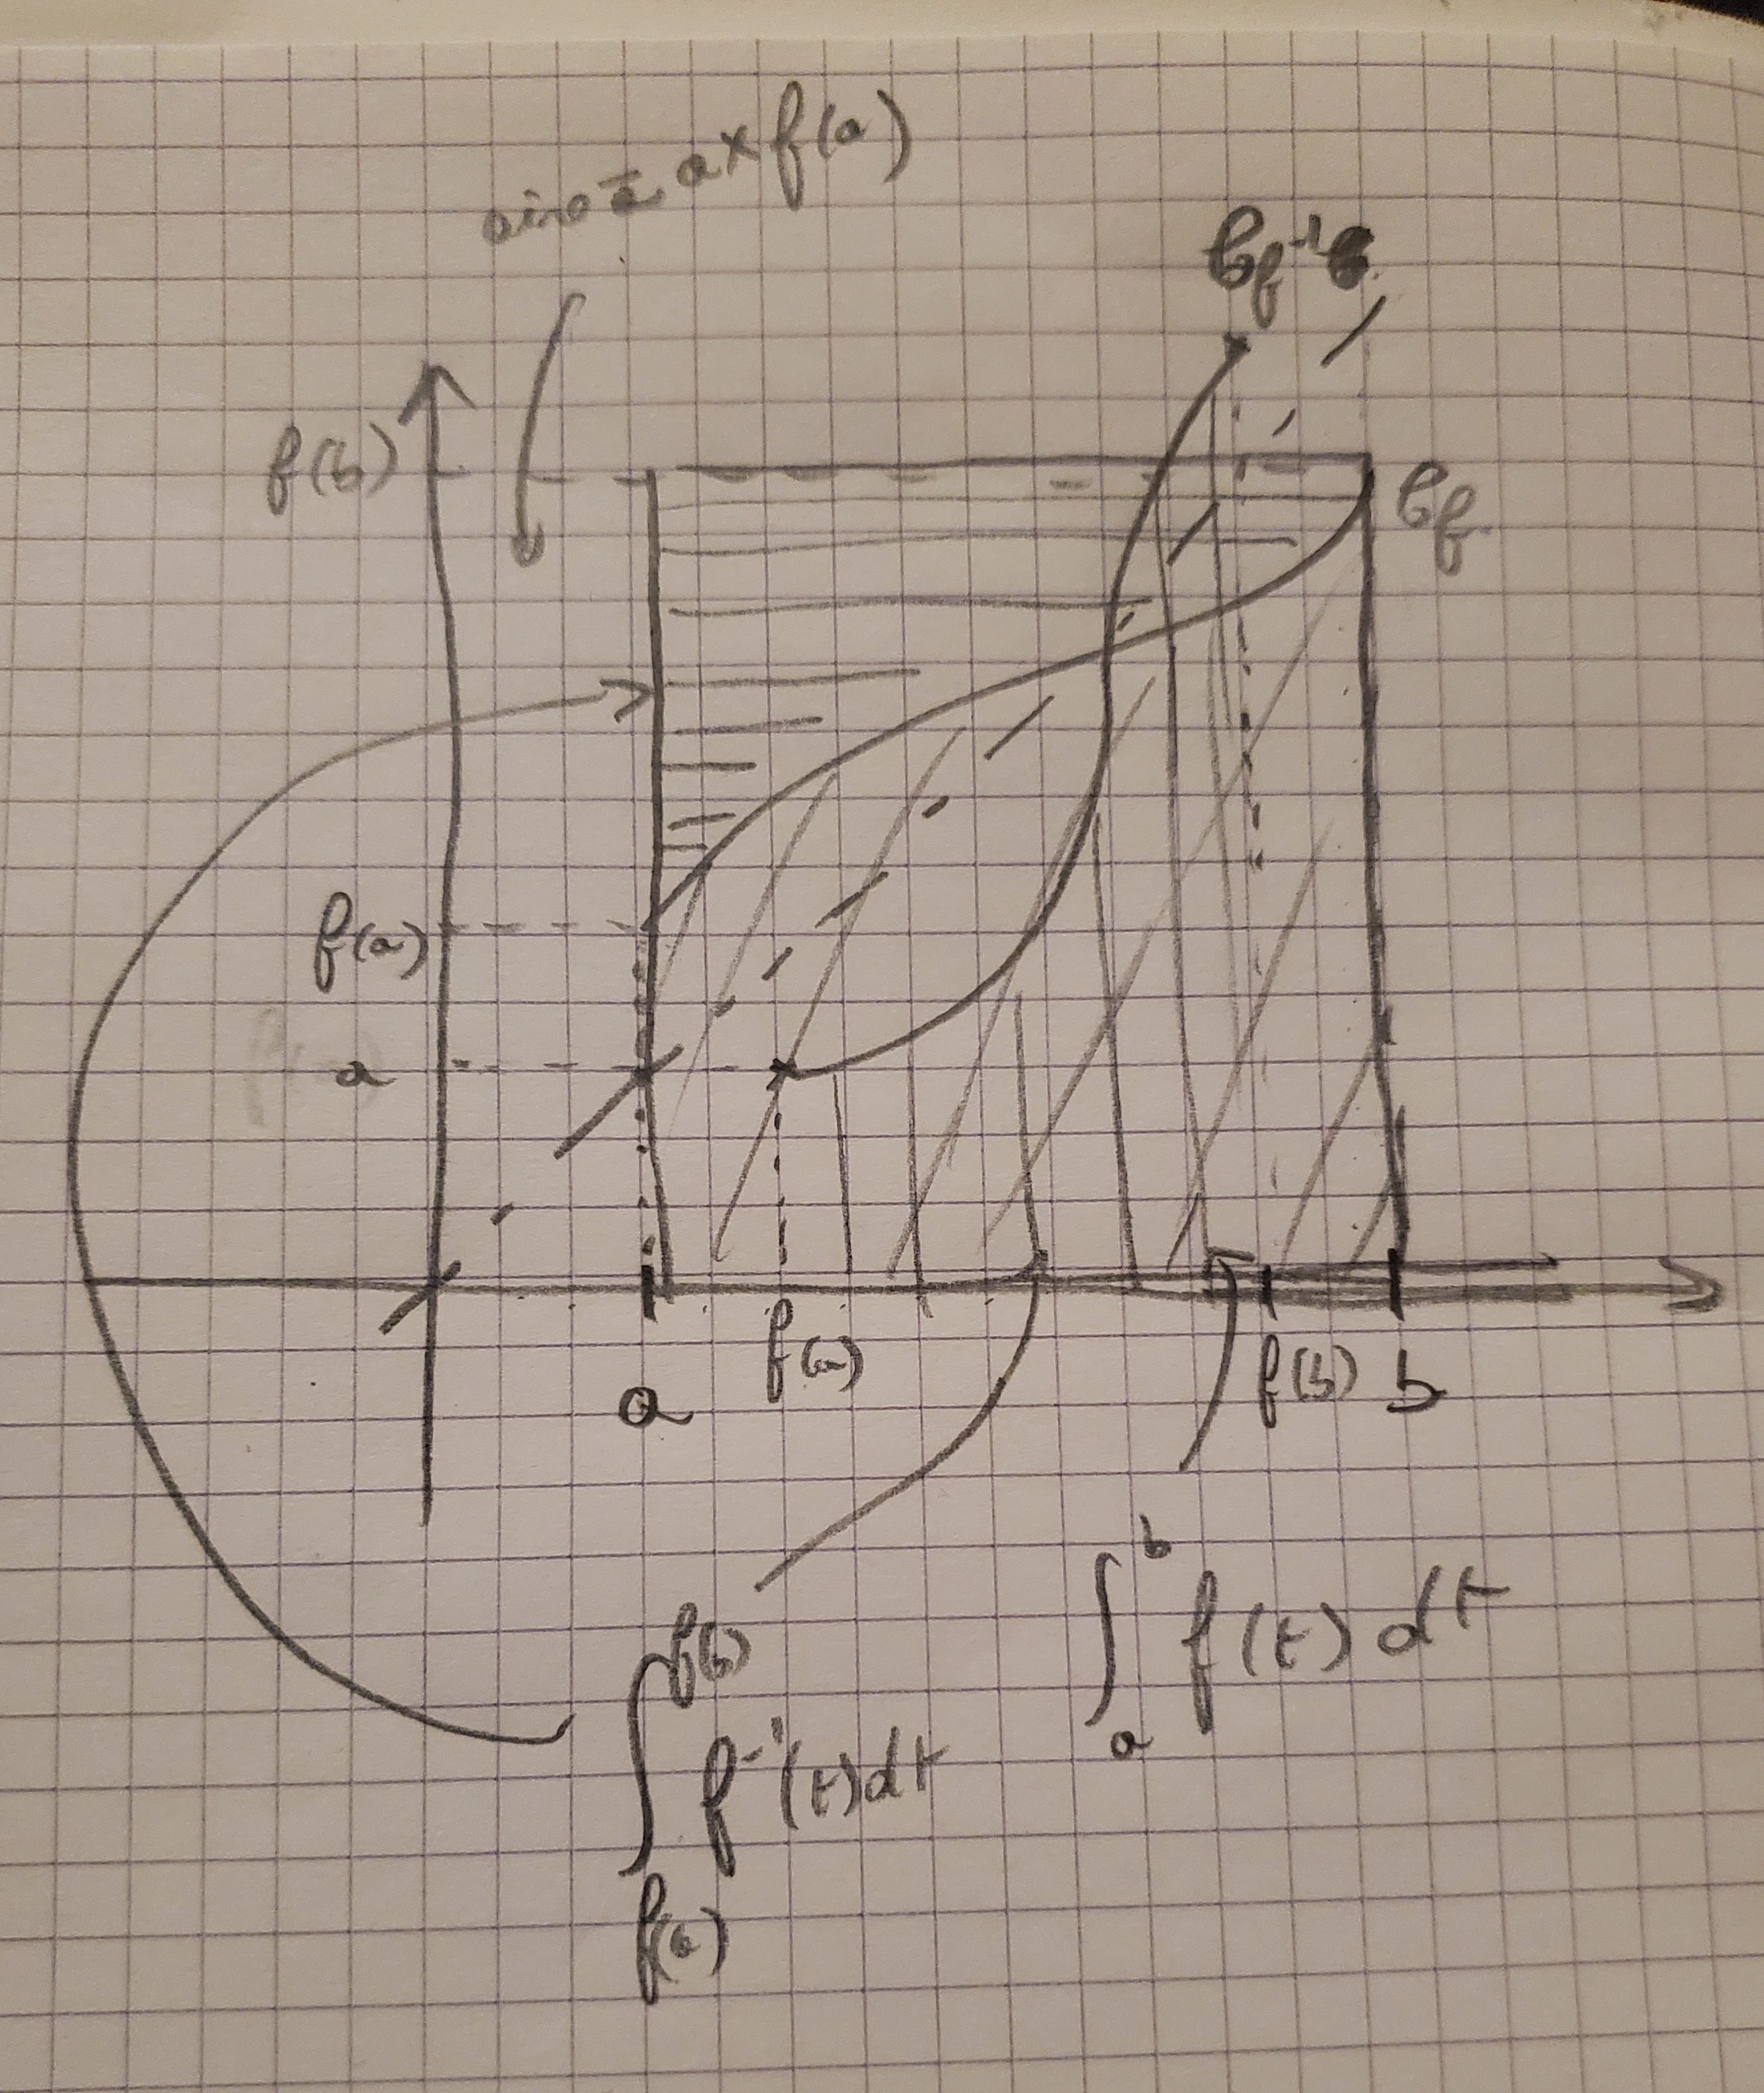
\includegraphics{./chapitres/integration/documents/propriete_geometrique.jpg}

\begin{center}
\begin{tikzpicture}[line cap=round, >=latex]

\begin{scope}[local bounding box=struct, scale=1]

    \def\u{0.5}
    \def\v{0.2}

    \def\xa{5}
    \def\ya{0.5}
    \def\xb{6.5}
    \def\yb{1.5}
    \def\xc{8}
    \def\yc{4}

    \path (\xa, \ya)    coordinate (A)
        (\xb, \yb)    coordinate (B)
        (\xc, \yc)  coordinate (C)
        (\ya, \xa)    coordinate (A')
        (\yb, \xb)    coordinate (B')
        (\yc, \xc)  coordinate (C');

    \begin{scope}
        \clip (A') ..controls +(0.05*\u, 0.05*\u) and ( $(B') + (-5*\v, -0.5*\u)$ )..
        (B') ..controls +(5*\v, 0.5*\u) and ( $(C') + (-2*\v, -2*\v)$ )..
        (C') |- cycle;
        %\clip (A') ..controls +(0.05*\u, 0.05*\u) and ( $(B') + (-0.5*\v, -0.5*\u)$ )..
        %(B') ..controls +(5*\v, 0.5*\u) and ( $(C') + (-2*\v, -2*\v)$ )..
        %(C') |- cycle;
        \foreach \x in {\ya00, \ya01,...,\yc.000}   
            \draw[blue!15!white, opacity=0.5] (\x,0) -- ++(0,8);
    \end{scope}

    \fill[blue!15!white] (\ya,0) rectangle ++(\yc-\ya,\xa);

    \begin{scope}
        \clip (A) ..controls +(0.05*\u, 0.05*\u) and ( $(B) + (-0.5*\u, -5*\v)$ )..
        (B) ..controls +(0.5*\u, 5*\v) and ( $(C) + (-2*\v, -2*\v)$ )..
            (C) |- cycle;
        \foreach \x in {\xa.000, \xa.001,...,\xc.000}   
            \draw[red!15!white, opacity=0.5] (\x,-\ya) -- ++(0,10);
    \end{scope}

    \draw[thick, blue] 
        (A') ..controls +(0.05*\u, 0.05*\u) and ( $(B') + (-5*\v, -0.5*\u)$ )..
        (B') ..controls +(5*\v, 0.5*\u) and ( $(C') + (-2*\v, -2*\v)$ )..
        (C') node[right] {$\mathcal{C}_f^{-1}$};
        
    \draw[thick, red] 
        (A) ..controls +(0.05*\u, 0.05*\u) and ( $(B) + (-0.5*\u, -5*\v)$ )..
        (B) ..controls +(0.5*\u, 5*\v) and ( $(C) + (-2*\v, -2*\v)$ )..
            (C) node[above] {$\mathcal{C}_f$};


    \fill[red!15!white] (\xa,0) rectangle ++(\xc-\xa,\ya);

    \draw[gray] (-.5, -.5) -- (\xc + 0.5, \xc.5) node[below left] {\contour{white}{\footnotesize$y = x$}};

    \draw[dashed] (\xa, 0) node[black,below]{\footnotesize$a$} -- (A);
    \draw[dashed] (0, \ya) node[black,left]{\footnotesize$f(a)$} -- (A);
    
    \draw[dashed] (\xc, 0) node[black,below]{\footnotesize$b$} -- (C);
    \draw[dashed] (0, \yc) node[black,left]{\footnotesize$f(b)$} -- (C);

    \draw[dashed] (0, \xa) node[black,left]{\footnotesize$a$} -- (A');
    \draw[dashed] (\ya, 0) node[black,below]{\footnotesize$f(a)$} -- (A');
    
    \draw[dashed] (0, \xc) node[black,left]{\footnotesize$b$} -- (C');
    \draw[dashed] (\yc, 0) node[black,below]{\footnotesize$f(b)$} -- (C');

    \draw[->, black] (5.5,2) node[above] 
    {\footnotesize \contour{white}{$\displaystyle \int_a^b f(t)\, \mathrm{d} t$}} to [out=-90,in=180] ($(7,1.5)$);

    % \draw[->, black] (3,-0.5) node[below] 
    % {\footnotesize \contour{white}{$\displaystyle \int_{f(a)}^{f(b)} f^{-1}(t)\, \mathrm{d} t$}} to [out=70,in=-70] ($(3,1.5)$);
    \node at ((2.5, 5) {\footnotesize \contour{blue!15!white}{$\displaystyle \int_{f(a)}^{f(b)} f^{-1}(t)\, \mathrm{d} t$}};

    \draw[thick, ->] (-.5, 0) -- (\xc + 0.5, 0) node[above] {$x$};
    \draw[thick, ->] (0, -.5) -- (0, \xc + 0.5) node[left] {$y$};

\end{scope}

\end{tikzpicture}
\end{center}
